\documentclass[border=4pt]{standalone}
\usepackage{amsmath,amssymb}
\usepackage{tikz}
\usetikzlibrary{arrows.meta}
\definecolor{cfg}{HTML}{2E7D46}\definecolor{mcfb}{HTML}{2166AC}\definecolor{negr}{HTML}{B03A2E}
\definecolor{inkc}{HTML}{1B1B1B}\definecolor{gy}{HTML}{6B7280}
\begin{document}
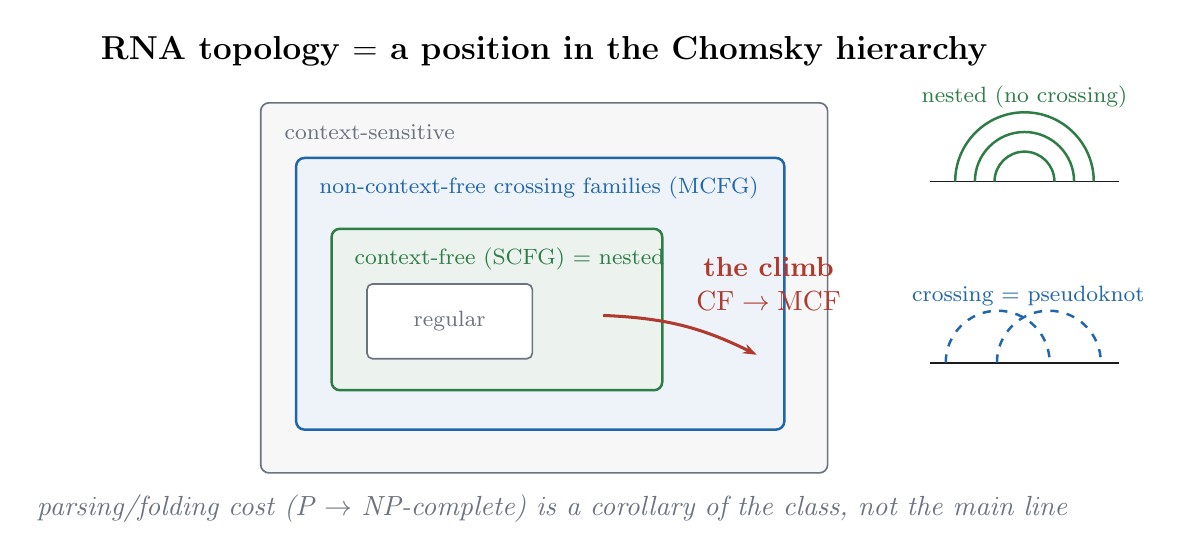
\begin{tikzpicture}[>={Stealth[length=5pt,width=3.6pt]}, font=\footnotesize]
\node[font=\large\bfseries] at (3.6,5.35) {RNA topology $=$ a position in the Chomsky hierarchy};
% nested containment: coloured regions (LRC-style)
\draw[rounded corners=3pt, gy, line width=0.6pt, fill=black!3] (0,0) rectangle (7.2,4.7);
\node[gy, anchor=north west] at (0.18,4.55) {context-sensitive};
\draw[rounded corners=3pt, mcfb, line width=0.9pt, fill=mcfb!8] (0.45,0.55) rectangle (6.65,4.0);
\node[mcfb, anchor=north west] at (0.62,3.88) {non-context-free crossing families (MCFG)};
\draw[rounded corners=3pt, cfg, line width=0.9pt, fill=cfg!9] (0.9,1.05) rectangle (5.1,3.1);
\node[cfg, anchor=north west] at (1.07,2.98) {context-free (SCFG) $=$ nested};
\draw[rounded corners=2pt, gy, line width=0.6pt, fill=white] (1.35,1.45) rectangle (3.45,2.4);
\node[gy] at (2.4,1.925) {regular};
% the climb
\draw[->, negr, line width=1.1pt] (4.35,2.0) to[bend left=12] (6.3,1.5);
\node[negr, font=\bfseries, align=center] at (6.45,2.4) {the climb\\$\mathrm{CF}\rightarrow\mathrm{MCF}$};
% arc cartoons
\draw[inkc, line width=0.6pt] (8.5,3.7)--(10.9,3.7);
\foreach \r in {0.38,0.63,0.88} \draw[cfg, line width=0.9pt] (9.7-\r,3.7) arc(180:0:\r);
\node[cfg] at (9.7,4.78) {nested (no crossing)};
\draw[inkc, line width=0.6pt] (8.5,1.4)--(10.9,1.4);
\draw[mcfb, line width=0.9pt, dashed] (8.7,1.4) arc(180:0:0.66);
\draw[mcfb, line width=0.9pt, dashed] (9.35,1.4) arc(180:0:0.66);
\node[mcfb] at (9.75,2.25) {crossing $=$ pseudoknot};
% corollary
\node[gy, font=\itshape] at (3.7,-0.45) {parsing/folding cost (P $\rightarrow$ NP-complete) is a corollary of the class, not the main line};
\end{tikzpicture}
\end{document}
